%#!uplatex main.tex

\section{Application}

In this section, we introduce advanced usage of IIS.

\subsection{Render internal area}

\begin{figure}[htbp]
  \center
  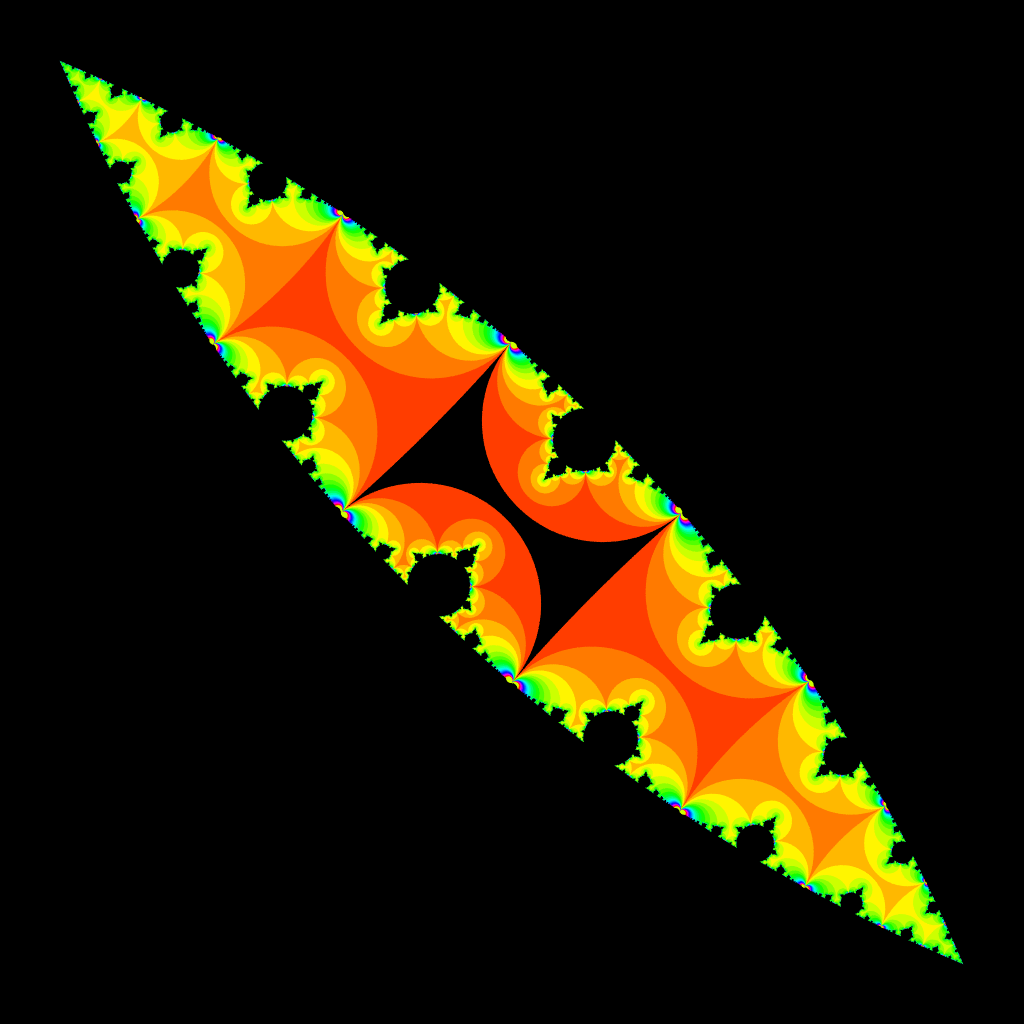
\includegraphics[height=1.35in, keepaspectratio]{img/application/internal/schottky.png}
  \caption{\textit{Edge of the circlte inversion fractal}}
  \label{fig:}
 \hspace*{\fill}
\end{figure}

%% 二次元のフラクタルの内側だけを描く.全ての円盤が接していれば極限集合
%% で二分割することができる

two dimensional circle inversion fractals

All of the circles touches each other, the limit set split plane by two.
transformed point is outside of the limit set.

\subsection{Render Edge of the Circles}

\begin{figure}[htbp]
  \center
  \includegraphics[height=1.35in, keepaspectratio]{img/application/edge/circleEdge.png}
  \caption{\textit{Edge of the circlte inversion fractal}}
  \label{fig:circleEdge}
 \hspace*{\fill}
\end{figure}

We can draw only edges of disks in circle inversion fractals.
We can estimate the distance from the center of the disks usin jacobian
of circle inversions.

%% ヤコビアンを累積させていき,最後の円周からの距離を累積させたヤコビア
%% ンで割ることで,円周から点までの距離を得ることができる.

\subsection{Geometrical Representation of M\"obius Transformation Groups}

%% メビウス変換を円や球の反転で定義することによって,より直観的に生成元
%% を得て描画することができる.

In this paper, we mainly use circle or sphere inversions.
We can compose M\"obius transformations by even number of their
inversion.


\subsubsection{Two Dimensionanl Generators}

\noindent\textbf{Inversion in a Circle with Infinite Radius.}

\noindent\textbf{Parallel Translation.}

\noindent\textbf{Rotation.}

\noindent\textbf{Composition of Two Circles.}

\noindent\textbf{Loxodromic.}


\subsubsection{Three Dimensionanl Generators}

\noindent\textbf{Inversion in a Sphere with Infinite Radius.}

\noindent\textbf{Parallel
Translation~\footnote{\url{https://www.shadertoy.com/view/lsjyzK}}.}

\noindent\textbf{Rotation.}

\noindent\textbf{Composition of Two Spheres~\footnote{\url{https://www.shadertoy.com/view/ldByDW}}.}

\noindent\textbf{Compound Loxodromic~\footnote{\url{https://www.shadertoy.com/view/MdjyRV}}.}

\subsection{Sphairahedra and Three-dimensional Fractals}

%% 球面体のタイリングもIISで描画することができる

Kazushi Ahara and Yoshiaki Araki invented \textit{Sphairahedron} in
2003.
Sphairahedron is coined word combining two words sphaira- and -hedron.